 % \begin{tikzpicture}[scale=0.8]
 %      \draw
 %        (-9.0, 0.0) node[fill=cyan, rounded corners] (0){Source}
 %        (-5.745, 1.085) node[fill=pink, rounded corners] (1){Cota}
 %        (-5.745, 0.0) node[fill=pink, rounded corners] (2){Cota}
 %        (-5.745, -1.085) node[fill=gray, rounded corners] (3){Resto}
 %        (0.766, 0.0) node[fill=brown, rounded corners] (4){$u$}
 %        (0.766, -1.085) node[fill=brown, rounded corners] (5){$u$}
 %        (0.766, 1.085) node[fill=brown, rounded corners] (6){$u$}
 %        (-2.489, 1.085) node[fill=yellow, rounded corners] (7){$p$}
 %        (-2.489, 0.0) node[fill=yellow, rounded corners] (8){$p$}
 %        (-2.489, -1.085) node[fill=yellow, rounded corners] (9){$p$}
 %        (4.021, 2.713) node[fill=orange, rounded corners] (10){$u$}
 %        (4.021, 1.628) node[fill=orange, rounded corners] (11){$u$}
 %        (4.021, 0.543) node[fill=orange, rounded corners] (12){$u$}
 %        (4.021, -0.543) node[fill=orange, rounded corners] (13){$u$}
 %        (4.021, -1.628) node[fill=orange, rounded corners] (14){$u$}
 %        (4.021, -2.713) node[fill=orange, rounded corners] (15){$u$}
 %        (7.277, 0.0) node[fill=cyan, rounded corners] (16){Target};
 %      \begin{scope}[-]
 %        \draw[lightgray, text=black, font=\footnotesize] (0) to node[] {0} (1);
 %        \draw[lightgray, text=black, font=\footnotesize] (0) to node[] {0} (2);
 %        \draw[lightgray, text=black, font=\footnotesize] (0) to node[] {0} (3);
 %        \draw[lightgray, text=black, font=\footnotesize] (1) to node[] {0} (7);
 %        \draw[lightgray, text=black, font=\footnotesize] (2) to node[] {0} (8);
 %        \draw[transparent] (3) to node[] {0 ; 0} (8);
 %        \draw[lightgray, text=black, font=\footnotesize] (3) to node[] {0} (9);
 %        \draw[transparent] (3) to node[] {0 ; 0} (7);
 %        \draw[lightgray, text=black, font=\footnotesize] (4) to node[] {0} (8);
 %        \draw[transparent] (4) to node[] {0 ; 4} (14);
 %        \draw[lightgray, text=black, font=\footnotesize] (4) to node[] {2} (13);
 %        \draw[transparent] (4) to node[] {0 ; 5} (12);
 %        \draw[transparent] (4) to node[] {0 ; 4} (11);
 %        \draw[lightgray, text=black, font=\footnotesize] (5) to node[] {0} (9);
 %        \draw[transparent] (5) to node[] {0 ; 4} (14);
 %        \draw[transparent] (5) to node[] {0 ; 2} (13);
 %        \draw[lightgray, text=black, font=\footnotesize] (5) to node[] {2} (15);
 %        \draw[transparent] (5) to node[] {0 ; 3} (11);
 %        \draw[lightgray, text=black, font=\footnotesize] (6) to node[] {0} (7);
 %        \draw[lightgray, text=black, font=\footnotesize] (6) to node[] {1} (10);
 %        \draw[transparent] (6) to node[] {0 ; 1} (14);
 %        \draw[lightgray, text=black, font=\footnotesize] (10) to node[] {0} (16);
 %        \draw[transparent] (11) to node[] {0 ; 0} (16);
 %        \draw[transparent] (12) to node[] {0 ; 0} (16);
 %        \draw[lightgray, text=black, font=\footnotesize] (13) to node[] {0} (16);
 %        \draw[transparent] (14) to node[] {0 ; 0} (16);
 %        \draw[lightgray, text=black, font=\footnotesize] (15) to node[] {0} (16);
 %      \end{scope}
 %    \end{tikzpicture}

\resizebox{0.7\textwidth}{!}{%
      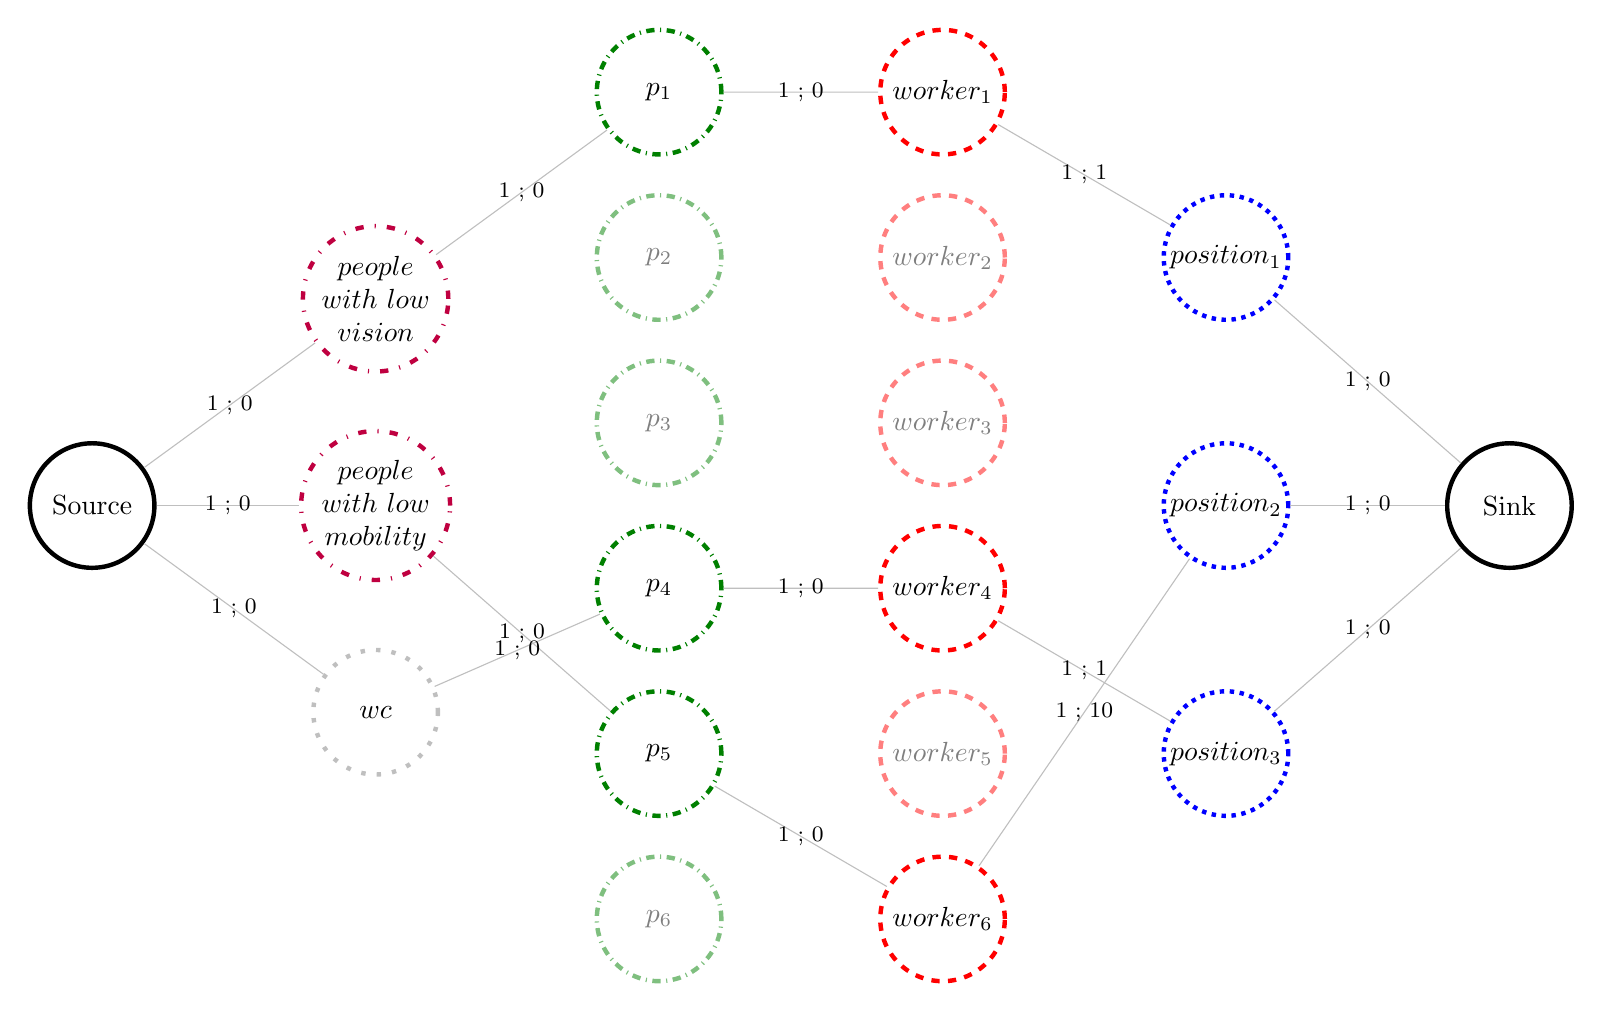
\begin{tikzpicture} [xscale=0.45, yscale=1.05]

      \tikzstyle{WC_style} = [circle, draw, fill, minimum size=45pt, inner sep=0pt, text centered, text width=1.5cm, align=center, font=\scriptsize]
        \tikzstyle{style} = [circle, draw, ultra thick, minimum size=45pt, inner sep=0pt, text centered]
            \tikzstyle{no_border} = [circle, ultra thick, minimum size=45pt, inner sep=0pt, text centered, opacity=0.5]
        
            \draw
              (-20.0, 0.0) node[draw=black,style] (0){Source}
              (-12.0, 2.5) node[draw=purple, loosely dashdotted, style, text width=1.5cm, align=center] (1){$people$ $with$ $low$ \\ $vision$}
              (-12.0, 0.0) node[draw=purple, loosely dashdotted, style, text width=1.5cm, align=center] (2){$people$ $with$ $low$ \\ $mobility$}
              (-12.0, -2.5) node[draw=lightgray, loosely dotted,style] (3){$wc$}
              (4.0, 5.0) node[draw=red, dashed,style] (4){$worker_1$}
              (4.0, 3.0) node[draw=red, dashed,no_border] (5){$worker_2$}
              (4.0, 1.0) node[draw=red, dashed,no_border] (6){$worker_3$}
              (4.0, -1.0) node[draw=red, dashed,style] (7){$worker_4$}
              (4.0, -3.0) node[draw=red, dashed,no_border] (8){$worker_5$}
              (4.0, -5.0) node[draw=red, dashed,style] (9){$worker_6$}
              (-4.0, 5.0) node[draw=green!50!black, dashdotted,style] (10){$p_1$}
              (-4.0, 3.0) node[draw=green!50!black, dashdotted,no_border] (11){$p_2$}
              (-4.0, 1.0) node[draw=green!50!black, dashdotted,no_border] (12){$p_3$}
              (-4.0, -1.0) node[draw=green!50!black, dashdotted,style] (13){$p_4$}
              (-4.0, -3.0) node[draw=green!50!black, dashdotted,style] (14){$p_5$}
              (-4.0, -5.0) node[draw=green!50!black, dashdotted,no_border] (15){$p_6$}
              (12.0, 3.0) node[draw=blue, dotted,style] (16){$position_1$}
              (12.0, -3.0) node[draw=blue, dotted,style] (17){$position_3$}
              (12.0, 0.0) node[draw=blue, dotted,style] (18){$position_2$}
              (20.0, 0.0) node[draw=black,style] (19){Sink};
        
      \begin{scope}[-]
        \draw[lightgray, text=black, font=\footnotesize] (0) to node[] {1 ; 0} (1);
        \draw[lightgray, text=black, font=\footnotesize] (0) to node[] {1 ; 0} (2);
        \draw[lightgray, text=black, font=\footnotesize] (0) to node[] {1 ; 0} (3);
        \draw[lightgray, text=black, font=\footnotesize] (1) to node[] {1 ; 0} (10);
        \draw[transparent] (1) to node[] {1 ; 0} (11);
        \draw[transparent] (1) to node[] {0 ; 0} (12);
        \draw[transparent] (2) to node[] {0 ; 0} (13);
        \draw[lightgray, text=black, font=\footnotesize] (2) to node[] {1 ; 0} (14);
        \draw[transparent] (3) to node[] {1 ; 0} (10);
        \draw[transparent] (3) to node[] {0 ; 0} (11);
        \draw[transparent] (3) to node[] {0 ; 0} (12);
        \draw[lightgray, text=black, font=\footnotesize] (3) to node[] {1 ; 0} (13);
        \draw[transparent] (3) to node[] {0 ; 0} (15);
        \draw[transparent] (3) to node[] {0 ; 0} (14);
        \draw[lightgray, text=black, font=\footnotesize] (4) to node[] {1 ; 0} (10);
        \draw[lightgray, text=black, font=\footnotesize] (4) to node[] {1 ; 1} (16);
        \draw[transparent] (5) to node[] {1 ; 0} (11);
        \draw[transparent] (5) to node[] {1 ; 7} (18);
        \draw[transparent] (6) to node[] {0 ; 0} (12);
        \draw[transparent] (6) to node[] {0 ; 7} (18);
        \draw[lightgray, text=black, font=\footnotesize] (7) to node[] {1 ; 0} (13);
        \draw[lightgray, text=black, font=\footnotesize] (7) to node[] {1 ; 1} (17);
        \draw[transparent] (8) to node[] {0 ; 0} (15);
        \draw[transparent] (8) to node[] {0 ; 10} (18);
        \draw[transparent] (8) to node[] {0 ; 10} (17);
        \draw[lightgray, text=black, font=\footnotesize] (9) to node[] {1 ; 0} (14);
        \draw[lightgray, text=black, font=\footnotesize] (9) to node[] {1 ; 10} (18);
        \draw[lightgray, text=black, font=\footnotesize] (16) to node[] {1 ; 0} (19);
        \draw[lightgray, text=black, font=\footnotesize] (17) to node[] {1 ; 0} (19);
        \draw[lightgray, text=black, font=\footnotesize] (18) to node[] {1 ; 0} (19);
      \end{scope}
    \end{tikzpicture}
    }%